\chapter{Experiments}

    The purpose of this chapter is to overview the experimentation phase of the project, which contains the work done to deploy and measure how applications behave when using either classic or \gls{alto}-guided solutions when faced with some of the constructed scenarios, that force some decision which impacts the underlying network.
    Whereas the developed unit tests in the implementation stage aim to verify the correct functionality of separate units of code pertaining to the system, the execution of the entire system as a whole to serve a set of hypothetical use cases can help achieve a better grasp on how correctly the system behaves .

    Adjacent to the goal of testing the system's behavior in an emulated environment, the experimentation phase also aims to embed in such environment a list of case study scenarios where applications could leverage the \gls{alto} system to their advantage, and subsequently observe and measure if and how the \gls{alto} server can help the client with its network insight that guide the client in taking application decisions that aim for a win-win scenario between the overlay and underlay.
    As comparison, other known application-network interaction strategies will also be observed and their results measured as a means to compare their impact in comparison to one that utilizes the implemented system.

    Findings on existing application-layer traffic optimization interactions and the proposal of the \gls{alto} protocol made on Chapter \ref{sec:state-of-art}, together with the specified system extensions on Chapter \ref{sec:specification} leads one to believe that a theoretical mutually beneficial scenario exists in an \gls{alto} approach that could not exist in one where only one of the layers gets all the input when applying traffic optimization decisions.
    This chapter, however, puts those theoretical scenarios into a practical environment that could be replicated by those reading this work, and exposing the created scenarios and collected data can corroborate the theoretical conclusions, as well as leaving an opportunity for future discussion on how the system behaved, including its performance, its success in aiding clients, other existing client options that could be a better route, system shortcomings, etc.
    In general, this discussion benefits the \gls{alto} project and can give more maturity to the system as it was put through multiple test scenarios against other common strategies.

    Section \ref{sec:experiments-technologies} displays the chosen technologies for tasks pertaining to the experiments.
    Section \ref{sec:experiments-setup} focuses on the required steps taken to setup the testing environment.
    This includes the design and deployment of a network topology to be emulated, the creation of mock applications to serve as clients for the system, and the design and deployment of application and network status measurement tools.
    Section \ref{sec:experiments-scenarios} follows with the individual overview of the devised scenarios to be executed, and with it experiment specifics such as the initial problem, what strategies will be tested to solve it, how many runs will be made per strategy, and what metrics will be measured.
    Finished the experiments, Section \ref{sec:experiments-results} will display the obtained results that were collected emulated environment, and Section \ref{sec:experiments-discussion} after that will discuss these results and how they fare with the theoretical findings.

\section{Technologies Used}

\label{sec:experiments-technologies}

    The \gls{core} \cite{core} was used as a network emulator and represents the backbone of the experiments as a whole as it will serve as the background for the running scenarios.
    This tool allows for the creation and emulation of network environments, and with it are included the abilities to construct network topologies and manipulate properties of the member nodes, which can include network routers, switches, and host machines, that will all be used for the designed experiment scenarios.
    Additionally, link connection properties can themselves be customized, as parameters like maximum bandwidth, packet loss percentage, or packet delay can be meticulously customized, and in fact will be in the upcoming scenarios as a means to simulate a given circumstance that may occur in a realistic environment, such as link inefficiency that results from peak traffic hours.
    Another property that was of great importance for the selection of \gls{core} on this work is that, on top of the virtual network environment, arbitrary code can be run on behalf of a given entity and can be addressed to another, acting as if it were an actual network.
    This will be leveraged to run software pre-packaged in the emulator, such as routing protocols that are essential for the correct expected behavior of a simulated network, but also to schedule software execution that was developed for this work, which includes the \gls{alto} server, network state providers - e.g., probing daemons and application feedback collectors - and system clients for the \gls{p2p} and \gls{http} mock applications that will be devised to play out a particular experiment scenario, and which will have embedded into it an \gls{alto} client to interface with the server for council.
    As the simulation tool runs on Linux and builds a simulated network that behaves very much like a real one, well known real-application tools can be used on top of it in other needed areas, including the deployment and measuring phases, which gives plenty of flexibility on tool selection.

    The execution of arbitrary code on the network nodes is accomplishes with the vcmd \cite{vcmd} tool, that runs the specified commands in control channels that are created at runtime by \gls{core} - for example, the following command executing a ping to address "10.0.0.1" with origins on node "P2P-Client-1", and on simulation session "12345":

    \begin{center}
    \begin{lstlisting}[caption=Execution of an example command through the control channel of a given node, language=bash]
$ vcmd -c /tmp/pycore.12345/P2P-Client-1 -- ping 10.0.0.1
    \end{lstlisting}
    \end{center}

    Python \cite{python} will be utilized to implement all simple software prototypes whose purpose is uniquely to test the application in a real scenario.
    This includes the \gls{p2p} file-transfer applications, the \gls{http} servers and clients, and the throughput-intensive activities done by the data servers.
    Appended to this programming language will also be the task of application monitoring, which includes the retrieval of performance statistics - doing so in the application's code itself, instead of using external tools, because more fine grained access exists and individual tasks can be monitored for how long and how well they perform.
    The choice of this language over others is simply that these software prototypes are not intended to be highly optimized, nor are they to be complex.
    Instead, their mode of operation is supposed to be simple in nature, to remove complex variables that might make the experiment results harder to infer upon, and to make reasoning and replication of experiment results easier.
    Python seems then like a good fit due to its easy syntax, its interpreted nature that skips work that would otherwise be needed for compilation that might increase performance - but is not required - and, finally, its massive collection of helpful libraries.


    Finally, for the task of network monitoring, to collect data representative of the impact that a given application strategy had in the infrastructure, the Linux file "/proc/net/dev" will be read in the virtual environment of each node, which contains the total amount of bytes that entered and left their interfaces during the scenario's run.
    Parsing all the data from each node and grouping them by area and \gls{as} is performed on a shell script, following the execution of the given scenario, and utilizing common text manipulation tools such as awk \cite{awk}.

\section{Setup}

\label{sec:experiments-setup}

    Figure \ref{fig:exp-topology} displays the topology that will act as the main environment for all the devised experiments, with partitioned views to be subsequently introduced.
    Figure \ref{fig:exp-global} presents a simplified global view the network as a collection of \glspl{as}.
    It was designed with the intent of reflecting, at a smaller scale, the structure of the Internet, in particular with it being an aggregation of multiple, heterogeneous, domains, each with their own topological properties and internal policies, with them being administrated by different organizations.
    A single backbone network, shown on Figure \ref{fig:exp-as0}, provides connectivity between many \glspl{as} and, to do its job correctly, a high degree of path redundancy exists between its routers, and the links have better capabilities than those associated with stub networks.
    Figure \ref{fig:exp-as1} shows \gls{as} 1, a simple topological structure consisting of five \glspl{pc} and three dedicated servers, connected with the help of switches and routers, that eventually connect to a single edge router that links with the backbone.
    Figure \ref{fig:exp-as2} shows \gls{as} 2, which is representative of a data center with two \gls{ospf} areas, both constructed with a hierarchical organization common for data center networks.
    Links in these regions are also highly capable and high traffic peak times are expected to occur.
    \gls{as} 3, shown in Figure \ref{fig:exp-as3}, is a slightly more complex stub network compared to \gls{as} 1, but has the same structure, with the addition of having three \gls{ospf} areas instead of one, and a variety of nodes and links with different properties - for example, the links in area A are generally better, whilst area C has wireless connections in it that are expected to have worse performance and be less reliable.
    Finally, \gls{as} 4, depicted on Figure \ref{fig:exp-as4}, connects directly with \gls{as} 3, meaning that it also acts as a transit \gls{as} to the rest of the network.
    Similarly to \gls{as} 3, it consists of a stub network accessed by many end users and some servers, and both node and link properties vary accordingly.

    \begin{figure}
    \centering
    \begin{subfigure}[t]{\textwidth}
    \centering
    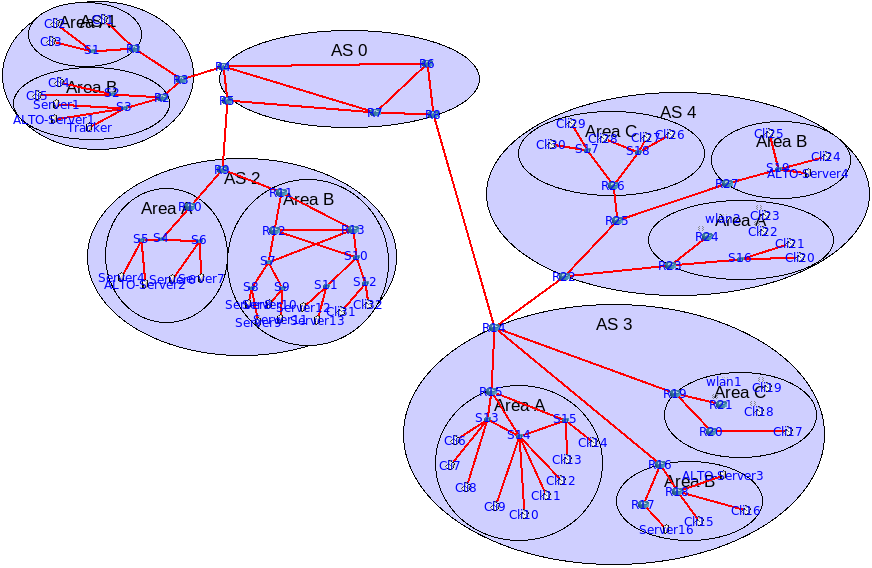
\includegraphics[scale=0.7]{img/topology-experiments-global.png}
    \caption{Global view of the network}    
    \label{fig:exp-global}
    \end{subfigure}

    \begin{subfigure}[t]{\textwidth}
    \centering
    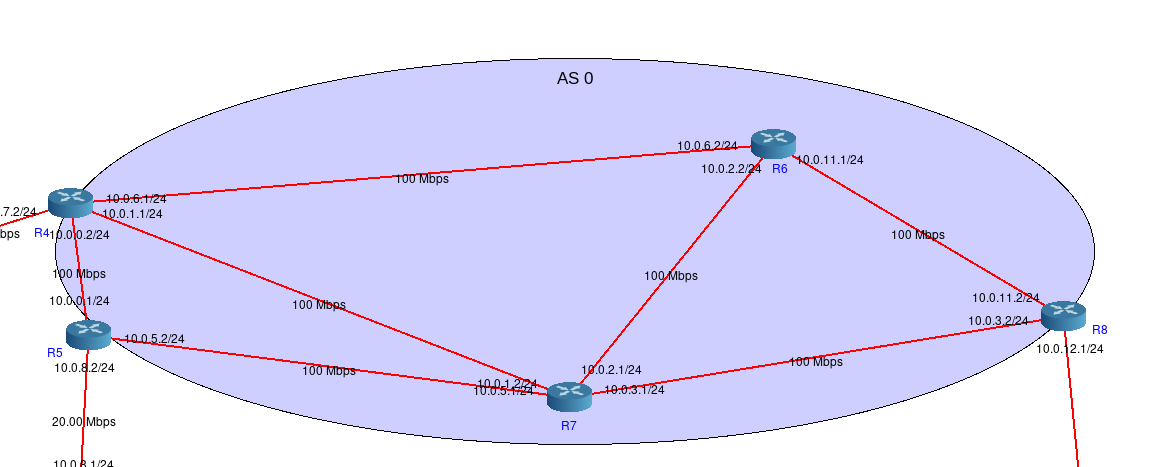
\includegraphics[scale=0.5]{img/topology-experiments-AS0.png}
    \caption{Detailed view of AS0}    
    \label{fig:exp-as0}
    \end{subfigure}

    \begin{subfigure}[t]{\textwidth}
    \centering
    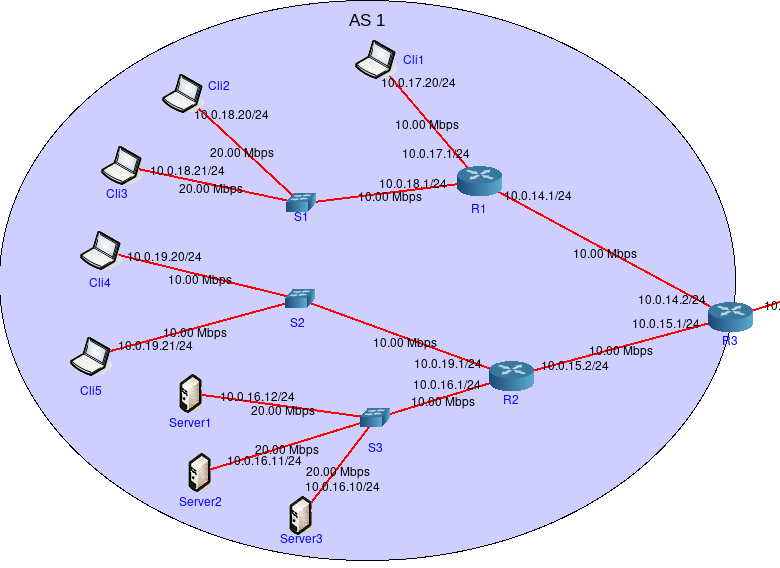
\includegraphics[scale=0.5]{img/topology-experiments-AS1.png}
    \caption{Detailed view of AS1}    
    \label{fig:exp-as1}
    \end{subfigure}
    \end{figure}

    \begin{figure} \ContinuedFloat
    \begin{subfigure}[t]{\textwidth}
    \centering
    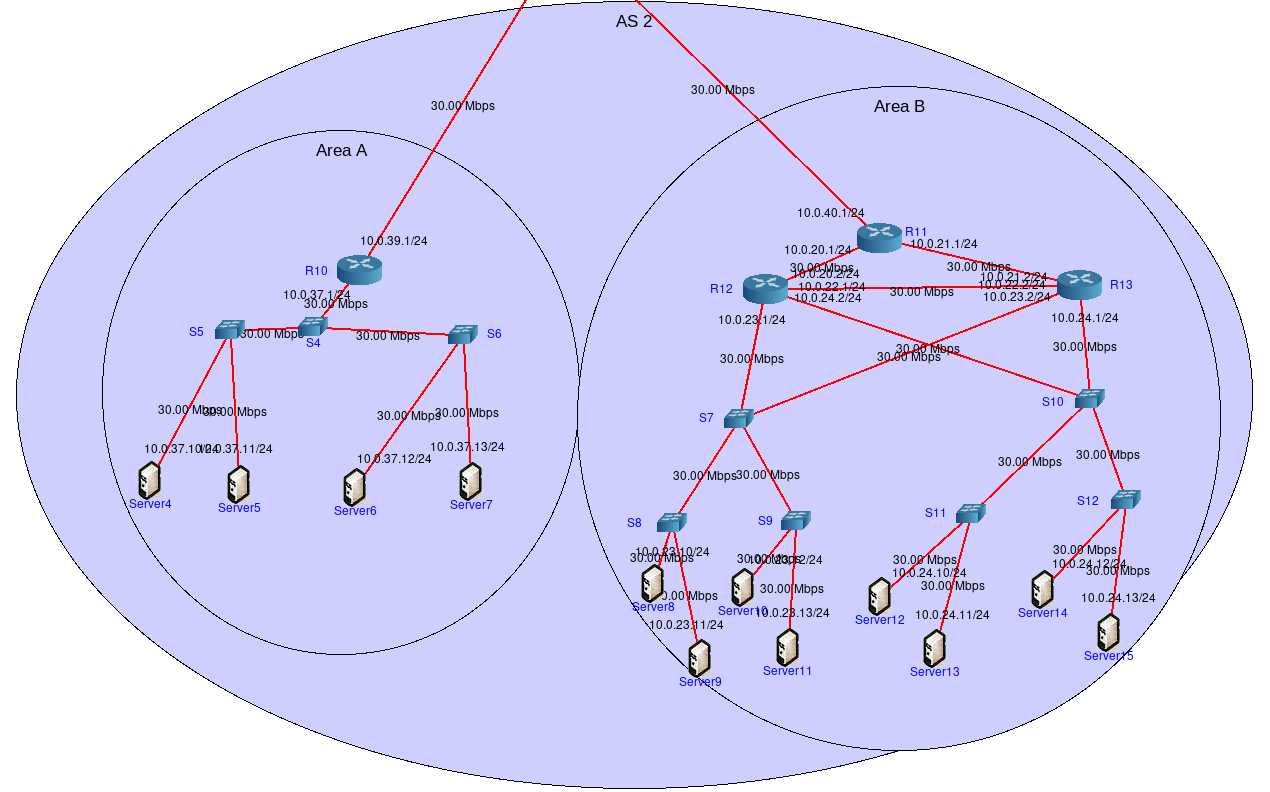
\includegraphics[scale=0.5]{img/topology-experiments-AS2.png}
    \caption{Detailed view of AS2}    
    \label{fig:exp-as2}
    \end{subfigure}

    \begin{subfigure}[t]{\textwidth}
    \centering
    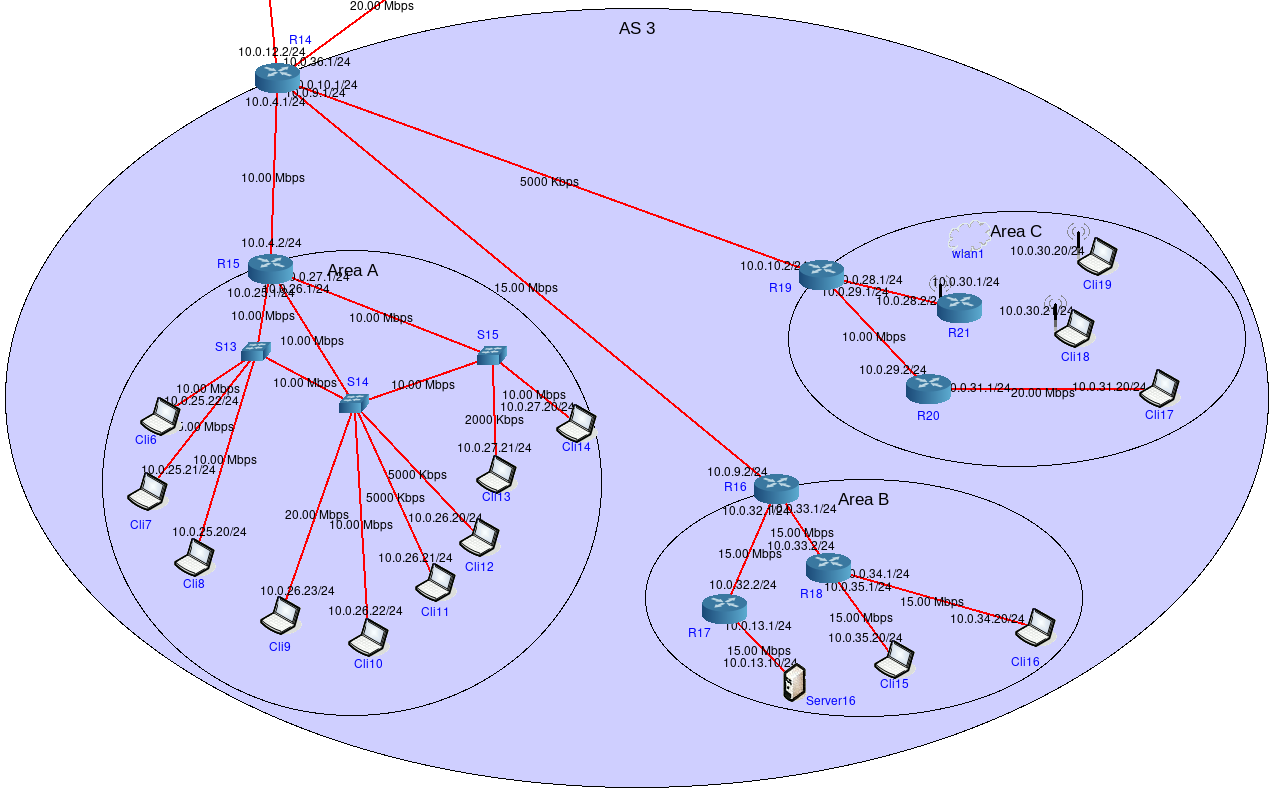
\includegraphics[scale=0.5]{img/topology-experiments-AS3.png}
    \caption{Detailed view of AS3}    
    \label{fig:exp-as3}
    \end{subfigure}
    \end{figure}

    \begin{figure} \ContinuedFloat
    \begin{subfigure}[t]{\textwidth}
    \centering
    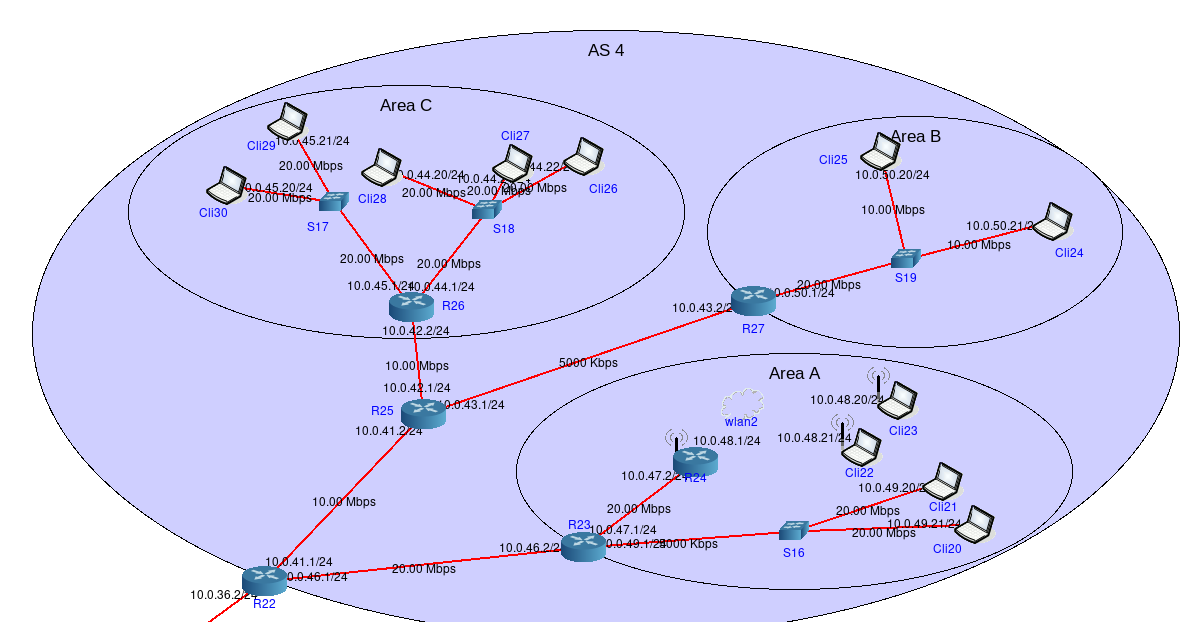
\includegraphics[scale=0.5]{img/topology-experiments-AS4.png}
    \caption{Detailed view of AS4}    
    \label{fig:exp-as4}
    \end{subfigure}

    \caption{Network topology and integrated \glspl{as}}
    \label{fig:exp-topology}
    \end{figure}


    Each node on the network has a given purpose that is represented as a node label, and link labels are used to specify connection properties.
    Unless stated otherwise with these labels, all other properties are equal throughout the network.
    Some pre-packaged \gls{core} services need to be enabled to assure network connectivity - mainly \gls{ospfv2} and \gls{bgp} - and scripting is used to, at the beginning of the simulation, bootstrap programs in specific nodes.

\section{Scenarios}

\label{sec:experiments-scenarios}

    This Section describes the three devised scenarios to test the impact to the overlay and underlay that results of applications performing traffic optimization decisions with and without the implemented \gls{alto} solution.
    Section \ref{ssec:scenario1} focuses on a \gls{p2p} application who needs to decide, whenever a file fragment is served by multiple peers, with whom to establish connection.
    Section \ref{ssec:scenario2} tackles the issue of an \gls{http} server subjected to periodic load spikes, and how clients can selectively choose the timing to initialize the resource request.
    Section \ref{ssec:scenario3} deals with the challenge of selecting a given \gls{http} server to retrieve a content from whenever a mirror cluster is available.

\subsection{Peer Selection in P2P File Transfer}

\label{ssec:scenario1}

\subsubsection{Overview}

    All nodes in the network labeled as "CliN", with N from 1 to 32, actively serve all ten equally sized fragments of a one gigabyte file to other peers, and the overlay bootstrapping method includes informing the tracker, labeled as "Tracker", about what file fragments they serve.

    "Cli2" wishes to retrieve the file, and to do so he firstly contacts the tracker for tracking information, which is given in the form of a file containing a mapping between each fragment \gls{id} and the available peers, alongside with the file's checksum for validation.

    Table \ref{table:fragment-allocations} shows what endpoints possess what file fragment IDs.
    For comparative reference, information is given about each fragment's location, i.e., the area and \gls{as} of the host serving it.
    Aditionally, the connection is also described with metrics from the perspective of the querying peer.
    These metrics include the maximum theoretical bandwidth as the minimum link bandwidth in the optimal path from Cli2 to each peer regarding this metric, and the sample \gls{rtt} measurement the client obtained after 10 sequential ping commands prior to the scenario's start.

\begin{table}[H]
\centering
\hspace*{-2.5em}
\begin{tabular}{|c|c|c|c|c|c|}
    \hline
    \textbf{Fragment ID} & \textbf{Endpoint} & \textbf{AS} & \textbf{Area} & \textbf{Max bandwidth (Mbps)} & \textbf{Sample RTT (ms)}  \\ \thickhline
   x00   & 10.0.18.21   & 1  &  A  & 20               & 0.172  \\ \hline
   x00   & 10.0.24.20   & 2  &  B  & 10               & 0.994  \\ \hline
   x00   & 10.0.35.20   & 3  &  B  & 10               & 1.174  \\ \thickhline

   x01   & 10.0.18.20   & 1  &  A  & resides locally  & 0.057  \\ \hline
   x01   & 10.0.26.21   & 3  &  A  & 5                & 1.236  \\ \hline
   x01   & 10.0.48.21   & 4  &  A  & 10               & 12.238 \\ \thickhline

   x02   & 10.0.19.21   & 1  &  B  & 10               & 0.846  \\ \hline
   x02   & 10.0.24.21   & 2  &  B  & 10               & 1.014  \\ \hline
   x02   & 10.0.35.20   & 3  &  B  & 10               & 1.174  \\ \thickhline

   x03   & 10.0.24.21   & 2  &  B  & 10               & 1.014  \\ \hline
   x03   & 10.0.27.21   & 3  &  A  & 2                & 1.661  \\ \hline
   x03   & 10.0.31.20   & 3  &  C  & 5                & 1.456  \\ \thickhline
    
   x04   & 10.0.18.21   & 1  &  A  & 20               & 0.172  \\ \hline
   x04   & 10.0.26.23   & 3  &  A  & 10               & 1.111  \\ \hline
   x04   & 10.0.24.20   & 2  &  B  & 10               & 0.994  \\ \thickhline

   x05   & 10.0.19.20   & 1  &  B  & 10               & 0.820  \\ \hline
   x05   & 10.0.24.20   & 2  &  B  & 10               & 0.994  \\ \hline
   x05   & 10.0.24.21   & 2  &  B  & 10               & 1.014  \\ \thickhline

   x06   & 10.0.27.21   & 3  &  A  & 2                & 1.661  \\ \hline
   x06   & 10.0.48.20   & 4  &  A  & 10               & 12.278 \\ \hline
   x06   & 10.0.49.21   & 4  &  A  & 5                & 1.260  \\ \thickhline

   x07   & 10.0.48.21   & 4  &  A  & 10               & 12.238 \\ \hline
   x07   & 10.0.49.21   & 4  &  A  & 5                & 1.260  \\ \hline
   x07   & 10.0.50.21   & 4  &  B  & 5                & 1.616  \\ \thickhline

   x08   & 10.0.50.20   & 4  &  B  & 5                & 1.627  \\ \hline
   x08   & 10.0.50.21   & 4  &  B  & 5                & 1.616  \\ \hline
   x08   & 10.0.35.20   & 3  &  B  & 10               & 1.174  \\ \thickhline

   x09   & 10.0.25.22   & 3  &  A  & 10               & 1.170  \\ \hline
   x09   & 10.0.26.21   & 3  &  A  & 5                & 1.236  \\ \hline
   x09   & 10.0.31.20   & 3  &  C  & 5                & 1.456  \\ \thickhline
\end{tabular}
\caption{Description of each fragment to be requested}
\label{table:fragment-allocations}
\end{table}

    After retrieveing the mapping, the client will sequencially request each fragment from its selected peer, finalizing with the merge all the fragments into a single file and the calculation of the checksum that will be compared with the one previously provided.

    An \gls{alto} server resides in the same \gls{as} and maintains resources - specifically, a local network map that groups peers within locality as "Area A" of "AS1", "Area B" of "AS2", or externally to "AS1".
    It also maintains global resources - specifically, an endpoint cost map indicating expected bandwidth and delay between all the peers participating in the overlay \gls{p2p} network.

    The variable actions to be tested are how the client selects which candidate peer, from the available pool, will be selected to serve a given file fragment.
    Table \ref{table:s1-tracker-methods} displays the different algorithms to be used.

\begin{table}[H]
\centering
\hspace*{-0.5em}
\begin{tabular}{|l|L|}
    \hline
    \textbf{Tracker Algorithm} & \multicolumn{1}{m{11cm}|}{\textbf{Description}}                                                                         \\ \hline
    Random                     & \multicolumn{1}{m{11cm}|}{Randomly elect among all available peers}                                                     \\ \hline
    RTT                        & \multicolumn{1}{m{11cm}|}{Select the peer with the smallest probe packet \gls{rtt} measurement average in 10 pings}     \\ \hline
    ALTO - Local               & \multicolumn{1}{m{11cm}|}{Retrieve the local network map from the requesting peer's \gls{alto} server and discover the peers whose \gls{pid} matches the requesting peer, choosing randomly if multiple options exist within that group}                                                                                                           \\ \hline
    ALTO - Global              & \multicolumn{1}{m{11cm}|}{Retrieve the global multicost endpoint cost map from the requesting peer's \gls{alto} server by selecting the \gls{tcp} throughput and one way delay metrics, and selecting the peer that maximizes throughput with a delay no bigger than 5 milliseconds.}                                                  \\ \hline
\end{tabular}
\caption{Peer selection algorithms to be tested in scenario 1}
\label{table:s1-tracker-methods}
\end{table}

    The experiment seeks to examine network resource usage and application performance for each algorithm.
    Table \ref{table:s1-measurements} presents the measurements that will be collected during the experiment runs.

\begin{table}[H]
\centering
\hspace*{-1.2em}
\begin{tabular}{|l|l|L|}
    \hline
    \textbf{Measurement}     & \textbf{Units}     & \multicolumn{1}{m{10cm}|}{\textbf{Description}}  \\ \hline
    Execution Time            & Seconds            & \multicolumn{1}{m{10cm}|}{Total amount of time required to select and retrieve all file fragments} \\ \hline
    Network Traffic          & Megabytes          & \multicolumn{1}{m{10cm}|}{Total amount inbound traffic to each network AS and area} \\ \hline
\end{tabular}
\caption{Measurements to be taken in scenario 1}
\label{table:s1-measurements}
\end{table}

\subsubsection{Analysis of Results}

Figure \ref{fig:graph-execution-scenario1} shows the execution times for each of the variable methods in this scenario.
It appears that the method of probing for path delay was the worst, at 1096 seconds of runtime, closely followed by the method of randomly selecting between the available peers.
Considerably faster are the \gls{alto}-related options.
The one considering a local server with its own information aided the application in achieving a 913.19 seconds execution time, whereas a global approach was able to considerably shave more time, at around 821.92 total seconds.

\begin{figure}[H]
\centering
\begin{tikzpicture}
    \begin{axis}[ 
        xbar,xmin=0,xmax=1500,
        xlabel={Execution times (s)},
        symbolic y coords={{ALTO-Global},{ALTO-Local},{RTT},{Random}},
        xtick={0, 500, 1000, 1500},
        ytick=data,
        nodes near coords, nodes near coords align={horizontal},
        ytick=data,
    ]
    \addplot[fill=lightblue] coordinates {(1096.314,{RTT}) (913.194,{ALTO-Local}) (821.915,{ALTO-Global}) (1052.820,{Random})};
    \end{axis}
\end{tikzpicture} %width=6cm,height=7.59cm
\caption{Execution times measured in scenario 1}
\label{fig:graph-execution-scenario1}
\end{figure}

    Figure \ref{fig:graph-traffic-scenario1} show the measured traffic influx into the network's \glspl{as} and their areas.
    It can be immediatelly identified that the delay probing method incurred in considerable amount of inbound traffic being generated, in all \glspl{as}.
    A random approach reduced that value significantly, in particular the amount of traffic that entered AS1 and its areas which were almost reduced in half, but the \gls{alto} approaches were both equally proficient and had the lowest amount of incoming traffic into AS1.
 
\begin{figure}[H]
\centering
\begin{tikzpicture}
    \pgfplotsset{%
        width=10cm,
        height=24cm
    }
    \begin{axis}[
        xbar,xmin=0,xmax=2500,
        bar width=8,
        xlabel={Traffic influx by region (bytes)},
        symbolic y coords={{ALTO-Global},{ALTO-Local},{RTT},{Random}},
        xtick={0, 500, 1000, 1500, 2000, 2500},
        enlarge y limits  = 0.2,
        enlarge x limits  = 0.01,
        typeset ticklabels with strut,
        legend pos=outer north east,
        ytick=data,
        nodes near coords, nodes near coords align={horizontal},
        ytick=data,
        reverse legend,
        legend image code/.code={
        \draw [#1] (0cm,-0.1cm) rectangle (0.5cm,0.1cm); }
    ]

    % Area 4 - Area C
    \addplot[fill=ao(english)] coordinates {(1.55280,{RTT}) (0.078516,{ALTO-Local}) (0.074514,{ALTO-Global}) (0.155280,{Random})};

    % Area 4 - Area B
    \addplot[fill=armygreen] coordinates {(2.817773,{RTT}) (0.077420,{ALTO-Local}) (0.074318,{ALTO-Global}) (2.817773,{Random})};

    % Area 4 - Area A
    \addplot[fill=applegreen] coordinates {(10.104310,{RTT}) (5.181086,{ALTO-Local}) (2.559743,{ALTO-Global}) (10.104310,{Random})};

    % AS 4
    \addplot[fill=green] coordinates {(12.763713,{RTT}) (5.177578,{ALTO-Local}) (2.556691,{ALTO-Global}) (5.058152,{Random})};

    % AS 3 - Area C
    \addplot[fill=canaryyellow] coordinates {(5.476332,{RTT}) (2.737291,{ALTO-Local}) (0.072710,{ALTO-Global}) (5.476332,{Random})};

    % AS 3 - Area B
    \addplot[fill=aureolin] coordinates {(5.424188,{RTT}) (0.077640,{ALTO-Local}) (2.707887,{ALTO-Global}) (5.424188,{Random})};

    % AS 3 - Area A
    \addplot[fill=bananayellow] coordinates {(5.133640,{RTT}) (2.562905,{ALTO-Local}) (5.045584,{ALTO-Global}) (5.133640,{Random})};

    % AS 3
    \addplot[fill=amber] coordinates {(28.322497,{RTT}) (10.322792,{ALTO-Local}) (10.159846,{ALTO-Global}) (12.840053,{Random})};

    % AS2 - Area B
    \addplot[fill=awesome] coordinates {(10.699966,{RTT}) (2.711305,{ALTO-Local}) (2.707281,{ALTO-Global}) (10.699966,{Random})};

    % AS2 - Area A
    \addplot[fill=alizarin] coordinates {(0.157304,{RTT}) (0.079984,{ALTO-Local}) (0.076102,{ALTO-Global}) (0.157304,{Random})};

    % AS2 
    \addplot[fill=red] coordinates {(10.697794,{RTT}) (2.709763,{ALTO-Local}) (2.707499,{ALTO-Global}) (7.993195,{Random})};

    % AS1 - Area B
    \addplot[fill=navy-blue] coordinates {(0.160326,{RTT}) (5.052812,{ALTO-Local}) (5.047120,{ALTO-Global}) (0.088108,{Random})};
    % AS1 - Area A
    \addplot[fill=lightblue] coordinates {(1710.524046,{RTT}) (798.246822,{ALTO-Local}) (798.246910,{ALTO-Global}) (912.287378,{Random})};
    % AS1
    \addplot[fill=blue] coordinates {(1711.189266,{RTT}) (570.387434,{ALTO-Local}) (570.421828,{ALTO-Global}) (912.733470,{Random})};

    \legend{AS4-AreaC, AS4-AreaB, AS4-AreaA, AS4, AS3-AreaC, AS3-AreaB, AS3-AreaA, AS3, AS2-AreaB, AS2-AreaA, AS2, AS1-AreaB, AS1-AreaA, AS1}
    \end{axis}
\end{tikzpicture}
\caption{Inbound traffic flux by network areas measured in Scenario 1}
\label{fig:graph-traffic-scenario1}
\end{figure}

    It seems like a random selection of peers, as was expected, was far from optimal for execution time. 
    Whilst random selection can be thought of as a good strategy to guarantee an even load distribution between peers, acting purely with this goal in mind is clearly not efficient in regards to network resources, as peers with worst network conditions can be chosen, and traffic can more often escape outside of network regions, as indeed was shown on the measurement of traffic that entered AS1, which meant a considerable amount of peers were selected outside of network regions. 
    Perhaps surprisingly, a method of peer selection based on probing measurements targeting packet delay performed worse in regards to execution time and traffic locality.
    It appears that, for this topology and this overlay network, message delay was a bad indicator of application speed performance, and it favored a lot of peers that resided outside of local regions.
    The \gls{alto} method revealed to be the most efficient at both runtime and traffic localization.
    A local approach was simple to implement, required input from only one \gls{isp} knowledge domain, and was able to get good time efficiency and very good traffic localization.
    The client had a prioritization mechanisms that favored area locality, followed by \gls{as} locality, and finally random choice if the prior criteria could not be fulfilled.
    The global approach had concrete information regarding available throughput and one way delay, but no strategy to localize traffic, instead maximizing throughput with delay that did not compromise its \gls{qos} levels.
    It appears, however, that there was a correlation between higher throughput and locality, and by focusing only on the former, the latter was automatically achieved. 
    This can be seen because the global approach managed to generate the same amount of inbound traffic to AS1 while simultaneously reducing execution time.

\subsection{HTTP resource request scheduling}

\label{ssec:scenario2}

\subsubsection{Overview}

    "Server1" acts as a server of \gls{http} content.
    "Cli1" wishes to retrieve a 500MB file from that server in one single session.
    The server is subjected to variable, random client loads that affect processing and storage power, and subsequently its ability to serve clients, as well as periodic traffic loads within the \gls{as} whenever the server clusters in that system enchange data between themselves for server redundancy and general synchronization.
    This will be translated in practice as the dynamic variation of the available bandwidth of the link directly connected to the server.
    This has direct impact on the theoretical maximum available bandwidth from "Cli1" to the server, whose chronological values are specified in \ref{table:server-delays}:

\begin{table}[H]
\centering
\begin{tabular}{|c|c|}
    \hline
    \textbf{Simulation time (s)}  & \textbf{Max bandwidth (Mbps)}  \\ \hline
    0 - 180            & 2                                         \\ \hline
    180 - 360          & 3                                         \\ \hline
    360 - 540          & 5                                         \\ \hline
    540 - $\infty$     & 10                                        \\ \hline
\end{tabular}
\caption{Dynamically applied client-server path delays in scenario 2}
\label{table:server-delays}
\end{table}

    The server administrator is aware of the request loads that the server is subjected to and has maintained historical observations that existed in the past, which allowed him to reasonably predict how these will impact the server's performance in the future by detecting peak usage times.
    The \gls{alto} server local to "Cli1" maintains a calendar cost map displaying the information mentioned in Table \ref{table:server-delays}, i.e., it informs the client about the expected available bandwidth in the present and future.

    The variable action to be tested is how the \gls{http} client selects when to initialize its content request with the server.
Table \ref{table:s2-client-methods} displays the different client algorithms that will be tested for the task of server request scheduling.

\begin{table}[H]
\begin{tabular}{|l|L|}
    \hline
    \textbf{Client Algorithm} & \multicolumn{1}{m{11cm}|}{\textbf{Description}}                                                                     \\ \hline
    Immediate                 & \multicolumn{1}{m{11cm}|}{Immediatelly request the resource from the server}                                        \\ \hline
    RTT                       & \multicolumn{1}{m{11cm}|}{Continuously probe the network to measure the existing maximum available bandwidth until that value reaches above 10 Mbps}                                                                                                                                                                          \\ \hline
    ALTO                      & \multicolumn{1}{m{11cm}|}{Retrieve a calendar cost map from the \gls{alto} server in AS2 of expected path delay to the server, and iniciate immediately when the available bandwidth is expected to be 10 Mbps}                                                                                    \\ \hline
\end{tabular}
\caption{Client algorithms to be tested in scenario 2}
\label{table:s2-client-methods}
\end{table}

\textbf{Measurements:} Table \ref{table:s2-measurements} presents the measurements that will be collected during the experiment runs.

\begin{table}[H]
\centering
\begin{tabular}{|l|l|L|}
    \hline
    \textbf{Measurement}        & \textbf{Units}     & \multicolumn{1}{m{7cm}|}{\textbf{Description}}                                                  \\ \hline
    Transfer Time               & Seconds            & \multicolumn{1}{m{7cm}|}{Total amount of time required to transfer the file}                    \\ \hline
    Network Traffic             & Megabytes          & \multicolumn{1}{m{7cm}|}{Total amount of traffic that passed through each area in AS1}  \\ \hline
\end{tabular}
\caption{Measurements to be taken in scenario 2}
\label{table:s2-measurements}
\end{table}

\subsubsection{Analysis of Results}

Figure \ref{fig:graph-execution-scenario2} shows the obtained transfer times for each of the variable methods in scenario 2.
It appears that the \gls{alto}-aided and delay-probing methods were equally circling a 640 second runtime, and an approach of immediately querying the server was faster, at 457.19 seconds.

\begin{figure}[H]
\centering
\begin{tikzpicture}
    \begin{axis}[ 
        xbar,xmin=0,xmax=1500,
        xlabel={Execution times (s)},
        symbolic y coords={{ALTO-Global},{RTT},{Immediate}},
        xtick={0, 500, 1000, 1500},
        ytick=data,
        nodes near coords, nodes near coords align={horizontal},
        ytick=data,
    ]
    \addplot[fill=lightblue] coordinates {(641.998,{RTT}) (457.186,{Immediate}) (636.456,{ALTO-Global})};
    \end{axis}
\end{tikzpicture} %width=6cm,height=7.59cm
\caption{Execution times measured in scenario 2}
\label{fig:graph-execution-scenario2}
\end{figure}

Figure \ref{fig:graph-traffic-scenario2} shows the measured traffic influx into the areas of AS1.
It appears that the method that used bandwidth probing mechanisms took a considerable traffic overhead compared to the other two alternatives.

\begin{figure}[H]
\centering
\begin{tikzpicture}
    \pgfplotsset{%
        width=10cm,
        height=24cm
    }
    \begin{axis}[
        xbar,xmin=0,xmax=700,
        xlabel={Traffic influx by region (bytes)},
        symbolic y coords={{ALTO-Global},{RTT},{Immediate}},
        xtick={0, 100, 200, 300, 400, 500, 600, 650, 700},
        enlarge y limits  = 0.2,
        enlarge x limits  = 0.01,
        typeset ticklabels with strut,
        legend pos=outer north east,
        ytick=data,
        nodes near coords, nodes near coords align={horizontal},
        ytick=data,
        reverse legend,
        legend image code/.code={
        \draw [#1] (0cm,-0.1cm) rectangle (0.5cm,0.1cm); }
    ]

    % Area 4 - Area C
    \addplot[fill=ao(english)] coordinates {(0.062080,{RTT}) (0.064590,{ALTO-Global}) (0.052496,{Immediate})};

    % Area 4 - Area B
    \addplot[fill=armygreen] coordinates {(0.062202,{RTT}) (0.064378,{ALTO-Global}) (0.052198,{Immediate})};

    % Area 4 - Area A
    \addplot[fill=applegreen] coordinates {(0.062950,{RTT}) (0.063576,{ALTO-Global}) (0.052334,{Immediate})};

    % AS 4
    \addplot[fill=green] coordinates {(0.061240,{RTT}) (0.061170,{ALTO-Global}) (0.052298,{Immediate})};

    % AS 3 - Area C 
    \addplot[fill=canaryyellow] coordinates {(0.062496,{RTT}) (0.062794,{ALTO-Global}) (0.053866,{Immediate})};
    % AS 3 - Area B 
    \addplot[fill=aureolin] coordinates {(0.064296,{RTT}) (0.063370,{ALTO-Global}) (0.055118,{Immediate})};
    % AS 3 - Area A 
    \addplot[fill=bananayellow] coordinates {(0.065532,{RTT}) (0.065106,{ALTO-Global}) (0.054766,{Immediate})};

    % AS 3
    \addplot[fill=amber] coordinates {(0.061992,{RTT}) (0.059772,{ALTO-Global}) (0.050814,{Immediate})};

    % AS2 - Area B
    \addplot[fill=awesome] coordinates {(0.064102,{RTT}) (0.064378,{ALTO-Global}) (0.056352,{Immediate})};

    % AS2 - Area A
    \addplot[fill=alizarin] coordinates {(0.064144,{RTT}) (0.065730,{ALTO-Global}) (0.054380,{Immediate})};

    % AS2 
    \addplot[fill=red] coordinates {(0.062908,{RTT}) (0.059772,{ALTO-Global}) (0.054064,{Immediate})};

    % AS1 - Area B
    \addplot[fill=navy-blue] coordinates {(12.495609,{RTT}) (12.465589,{ALTO-Global}) (12.405077,{Immediate})};
    % AS1 - Area A
    \addplot[fill=lightblue] coordinates {(570.188334,{RTT}) (570.188204,{ALTO-Global}) (570.231908,{Immediate})};
    % AS1
    \addplot[fill=blue] coordinates {(0.066468,{RTT}) (0.066322,{ALTO-Global}) (0.059374,{Immediate})};

    \legend{AS4-AreaC, AS4-AreaB, AS4-AreaA, AS4, AS3-AreaC, AS3-AreaB, AS3-AreaA, AS3, AS2-AreaB, AS2-AreaA, AS2, AS1-AreaB, AS1-AreaA, AS1}
    \end{axis}
\end{tikzpicture}
\caption{Inbound traffic flux by network areas measured in scenario 2}
\label{fig:graph-traffic-scenario2}
\end{figure}

    It seems to be that, unsurprisingly, query timing had a big impact on total file transfer time, as these would set the available bandwidth during file transfer.
    Both the probing and \gls{alto}-aided strategies were able to correctly identify when the server was least overwhelmed by other clients, which justified their improved time results in comparison to immediately querying the server.
    However, these do not have similar network impacts.
    Firstly, the maximum bandwidth measuring approach required that the server hosted a measuring tool that the client could query to deduce network behavior, and this is a luxury that does not exist in most real-case scenarios.
    Secondly, deducing that information without \gls{isp} input required that a massive amount of overhead data be generated on a network, that not only used network resources in a sub-optimal manner, but it also added to the increase of the server's already overloaded capacity, which would, in a real-case scenario, further decrease the server's ability to handle client requests. 
    One could note that, in alternative to continuously probing the network, the client could use some exponential backoff strategy as to space out consecutive probing measurements, but that would, at the very least, generate an undesirable amount of overhead traffic, and could never be more quick than retrieving historical server pattern information from a reliable source.
    This last method was exactly what the \gls{alto} approach did, which was able to nullify any need to generate overhead traffic besides a very small request for the \gls{alto} resource, and simply waited to retrieve the content when the server was most available to, benefiting both sides and improving to a more sustainable server-client architecture and the health of the entire network.

\subsection{HTTP mirror selection}

\label{ssec:scenario3}

\subsubsection{Overview}

    "Cli2" wishes to retrieve a 500 megabyte file from a server.
    After querying the public proxy, an index is provided which contains a address lists of the four mirror servers that provide that content.
    The listing is show in table \ref{table:server-mirrors}.
    For comparative reference, information is given about each mirror's location, i.e., the area and \gls{as} where they reside.
    Additionally, the connection is also described with metrics from the perspective of the querying client. 
These metrics include the maximum theoretical bandwidth as the minimum link bandwidth in the optimal path from "Cli2" to each server regarding this metric, and the sample \gls{rtt} measurement the client obtained after 10 sequential ping commands prior to the scenario's start.

\begin{table}[H]
\centering
\begin{tabular}{|l|c|c|}
    \hline
    \textbf{Server address} & \textbf{AS} & \textbf{Area} & \textbf{Max bandwidth(Mbps) & Sample RTT (ms) } \\ \hline
    10.0.16.12              & 1           & B   &   &     \\ \hline
    10.0.37.10              & 2           & A   &   &     \\ \hline
    10.0.23.11              & 2           & B   &   &     \\ \hline
    10.0.13.10              & 3           & B   &   &     \\ \hline
\end{tabular}
\caption{Available server mirrors in scenario 3}
\label{table:server-mirrors}
\end{table}

The mirror servers will be subjected to constant loads at the start of the scenario, which are translated as throughput throttling applied from the client to the servers, which are specifically the ones shown in \ref{table:mirrors-bandwidth}.

\begin{table}[H]
\centering
\begin{tabular}{|l|c|}
    \hline
    \textbf{Server address} & \textbf{Throughput (Mbps)} \\ \hline
    10.0.16.12              & 3.0  Mbps                  \\ \hline
    10.0.37.10              & 5.0  Mbps                  \\ \hline
    10.0.23.11              & 10.0 Mbps                  \\ \hline
    10.0.13.10              & 5.0  Mbps                  \\ \hline
\end{tabular}
\caption{Client transference throttling to be applied if he chooses each given mirror server in scenario 3}
\label{table:mirrors-bandwidth}
\end{table}

    The \gls{alto} server local to that client provides a global \gls{alto} endpoint property map that contains \gls{cpu} and \gls{ram} load information about all the mirrors, as well as an endpoint cost map containing information about the expected bandwidth and delay from the client to the mirror.

    The variable action to be tested is how the \gls{http} client selects which mirror server to retrieve the file from.
    Table \ref{table:s3-client-methods} displays the different client algorithms that will be tested for the task of mirror selection.

\begin{table}[H]
\centering
\begin{tabular}{|l|L|}
    \hline
    \textbf{Client Algorithm} & \multicolumn{1}{m{11cm}|}{\textbf{Description}}                                                                                                               \\ \hline
    Random                    & \multicolumn{1}{m{11cm}|}{Randomly select a server }                                                                                                          \\ \hline
    Bandwidth                 & \multicolumn{1}{m{11cm}|}{Probe the mirrors for available TCP throughput and existing \gls{rtt}, and select the one with most bandwidth whose delay doesn't cross 2ms}   \\ \hline
    ALTO                      & \multicolumn{1}{m{11cm}|}{Retrieve an endpoint property map and endpoint cost map from the local \gls{alto} server, and choose the one with most available bandwidth and delay below 2ms, whose memory and processing power is below 30\%} \\ \hline
\end{tabular}
\caption{Client algorithms to be tested in scenario 3}
\label{table:s3-client-methods}
\end{table}

\textbf{Measurements:} Table \ref{table:s3-measurements} presents the measurements that will be collected during the experiment runs.

\begin{table}[H]
\centering
\begin{tabular}{|l|l|L|}
    \hline
    \textbf{Measurement}        & \textbf{Units}     & \multicolumn{1}{m{7cm}|}{\textbf{Description}}                                                  \\ \hline
    Transfer Time               & Seconds            & \multicolumn{1}{m{7cm}|}{Total amount of time required to transfer the file}                    \\ \hline
    Network Traffic             & Megabytes          & \multicolumn{1}{m{7cm}|}{Total amount of traffic that passed through each area network and AS}  \\ \hline
\end{tabular}
\caption{Measurements to be taken in scenario 3}
\label{table:s3-measurements}
\end{table}

\subsubsection{Analysis of Results}

Figure \ref{fig:graph-execution-scenario3} shows the obtained execution times for each of the variable methods in scenario 3.
An approach of randomly choosing mirror servers had the worst performance time wise, with 912.39 seconds, and the \gls{tcp} throughput measuring method following with 496.57 seconds.
Finally, the \gls{alto}-aided approach was the quickest with 456.21 seconds of runtime.

\begin{figure}[H]
\centering
\begin{tikzpicture}
    \begin{axis}[ 
        xbar,xmin=0,xmax=1200,
        xlabel={Execution times (s)},
        symbolic y coords={{ALTO-Global},{Bandwidth},{Random}},
        xtick={0, 500, 1000, 1200},
        ytick=data,
        nodes near coords, nodes near coords align={horizontal},
        ytick=data,
    ]
    \addplot[fill=lightblue] coordinates {(456.212,{ALTO-Global}) (496.567,{Bandwidth}) (912.394,{Random})};
    \end{axis}
\end{tikzpicture} %width=6cm,height=7.59cm
\caption{Execution times measured in scenario 3}
\label{fig:graph-execution-scenario3}
\end{figure}

Figure \ref{fig:graph-traffic-scenario3} shows the measured traffic influx into the network's \glspl{as} and their areas.
It appears that the approach that probed for path bandwidth had a considerable impacts on the generated traffic influx, and the spikes of traffic in the random and \gls{alto} approach give clues into the selected mirrors - those residing in AS3-B and AS2-B, most specifically.

\begin{figure}[H]
\centering
\begin{tikzpicture}
    \pgfplotsset{%
        width=10cm,
        height=24cm
    }
    \begin{axis}[
        xbar,xmin=0,xmax=700,
        enlarge y limits  = 0.2,
        enlarge x limits  = 0.01,
        xlabel={Traffic influx by region (bytes)},
        symbolic y coords={{ALTO-Global},{Bandwidth},{Random}},
        xtick={0, 100, 200, 300, 400, 500, 600, 650, 700},
        typeset ticklabels with strut,
        legend pos=outer north east,
        nodes near coords, nodes near coords align={horizontal},
        ytick=data,
        reverse legend,
        legend image code/.code={
        \draw [#1] (0cm,-0.1cm) rectangle (0.5cm,0.1cm); }
    ]
    % AS 4 - Area C
    \addplot[fill=ao(english)] coordinates {(0.075912,{Random}) (0.055872,{Bandwidth}) (0.053384,{ALTO-Global})};

    % AS 4 - Area B
    \addplot[fill=armygreen] coordinates {(0.076426,{Random}) (0.055142,{Bandwidth}) (0.053358,{ALTO-Global})};

    % AS 4 - Area A
    \addplot[fill=applegreen] coordinates {(0.076176,{Random}) (0.054574,{Bandwidth}) (0.053664,{ALTO-Global})};

    % AS 4
    \addplot[fill=green] coordinates {(0.074608,{Random}) (0.054080,{Bandwidth}) (0.052362,{ALTO-Global})};

    % AS3 - Area C
    \addplot[fill=canaryyellow] coordinates {(0.077134,{Random}) (0.055872,{Bandwidth}) (0.054750,{ALTO-Global})};

    % AS3 - Area B
    \addplot[fill=aureolin] coordinates {(13.350893,{Random}) (0.055142,{Bandwidth}) (0.054312,{ALTO-Global})};

    % AS3 - Area A
    \addplot[fill=bananayellow] coordinates {(0.079726,{Random}) (0.058132,{Bandwidth}) (0.054394,{ALTO-Global})};

    % AS 3
    \addplot[fill=amber] coordinates {(13.348379,{Random}) (6.415429,{Bandwidth}) (0.051206,{ALTO-Global})};

    % AS2 - Area B
    \addplot[fill=awesome] coordinates {(0.078224,{Random}) (12.585748,{Bandwidth}) (13.202365,{ALTO-Global})};

    % AS2 - Area A
    \addplot[fill=alizarin] coordinates {(0.078416,{Random}) (25.785258,{Bandwidth}) (0.055618,{ALTO-Global})};

    % AS2 
    \addplot[fill=red] coordinates {(0.077014,{Random}) (38.313674,{Bandwidth}) (13.200761,{ALTO-Global})};

    % AS1 - Area B
    \addplot[fill=navy-blue] coordinates {(0.080092,{Random}) (12.585188,{Bandwidth}) (0.056120,{ALTO-Global})};
    % AS1 - Area A
    \addplot[fill=lightblue] coordinates {(570.197962,{Random}) (571.161868,{Bandwidth}) (570.178424,{ALTO-Global})};
    % AS1
    \addplot[fill=blue] coordinates {(570.196112,{Random}) (571.481703,{Bandwidth}) (570.709008,{ALTO-Global})};

    \legend{AS4-AreaC, AS4-AreaB, AS4-AreaA, AS4, AS3-AreaC, AS3-AreaB, AS3-AreaA, AS3, AS2-AreaB, AS2-AreaA, AS2, AS1-AreaB, AS1-AreaA, AS1}
    \end{axis}
\end{tikzpicture}
\caption{Inbound traffic flux by network areas measured in scenario 3}
\label{fig:graph-traffic-scenario3}
\end{figure}

    Regarding scenario 3, it seems like the random mirror selection had the worst runtime, probably due to the fact that most of the servers were under load, and randomly selecting the best one, over many runs, was unlikely.
    A throughput probing approach was able to select the most apt mirror server to provide the server, but at the expense of much traffic overhead required to deduce available throughput.
    Additionally, this approach required from all mirror servers the hosting of a probing server that made these measurements possible, a luxury not possible in much real-case scenarios.
    The \gls{alto} approach was able to get immediate \gls{isp} input in the form of a combined multi-\gls{alto} domain effort, and quickly query the optimal mirror, resulting in a slightly better runtime than a probing approach.
